\ifdefined\standalone 
\documentclass[12pt]{article}
\usepackage{graphicx}
\usepackage{float}
\usepackage[a4paper, margin=1in]{geometry}
\usepackage[utf8]{inputenc}
\usepackage{textcomp}
\usepackage{amsmath}
\usepackage{booktabs}
\usepackage{tikz}
\usepackage{enumitem}
\usetikzlibrary{decorations.pathmorphing,patterns}
\usepackage[hidelinks]{hyperref} % <- hypertext

\begin{document}
\fi

\section{Fixed temperatures at boundaries}

A slab of thickness $L = 10~\mathrm{cm}$ is considered. Constant temperatures are imposed at the boundaries, with a temperature of $T_{\infty,t} = 400~^\circ\mathrm{C}$ at the top surface and $T_{\infty,b} = 20~^\circ\mathrm{C}$ at the bottom surface. The initial temperature of the slab is $T_{ini}=0~^\circ\mathrm{C}$, as illustrated in Figure~\ref{fig:ref_fixed_configuration}. The thermophysical properties of the material used in the simulation are reported in Table~\ref{tab:phys_props_fixed}.

The numerical results are validated against the analytical solution given by Incropera et al.~\cite{incropera_fundamentals_2007}. The analytical temperature distribution is expressed as:
\begin{equation}
T(z,t) = T_{\mathrm{ss}}(z) + \sum_{n=1}^{\infty} 
C_n \sin\left( \frac{n \pi z}{L} \right) 
\exp\left[ - \alpha \left( \frac{n \pi}{L} \right)^2 t \right]
\label{eq:T_xt_fixed_bc}
\end{equation}
where the steady-state temperature profile is
\begin{equation}
T_{\mathrm{ss}}(z) = T_{\infty,t} + \frac{T_{\infty,b} - T_{\infty,t}}{L}\, z
\end{equation}
and the Fourier coefficients are given by
\begin{equation}
C_n = \frac{2}{n\pi} 
\left[ 
(T_{ini} - T_{\infty,t}) + (T_{ini} - T_{\infty,b})(-1)^{n+1} 
\right]
\label{eq:Cn}
\end{equation}
Here, $T_0$ denotes the initial uniform temperature of the slab, and $\alpha = k / (\rho c_p)$ is the thermal diffusivity.

 A comparison between numerical and analytical temperature profiles is presented in Figure~\ref{fig:ref_fixed_temp}.

\begin{table}[H]
\centering
\caption{Thermophysical properties of the slab material}
\label{tab:phys_props_fixed}
\renewcommand{\arraystretch}{1.3}
\begin{tabular}{c c c c}
\hline
$k$ ($\mathrm{W\,m^{-1}\,K^{-1}}$) & 
$c_p$ ($\mathrm{J\,kg^{-1}\,K^{-1}}$) & 
$\rho$ ($\mathrm{kg\,m^{-3}}$) & 
$\varepsilon$ ($-$) \\
\hline
0.10 & 1000 & 100 & 0.0 \\
\hline
\end{tabular}
\end{table}

\begin{figure}[H]
\centering
\begin{minipage}[t]{0.45\textwidth}
\centering
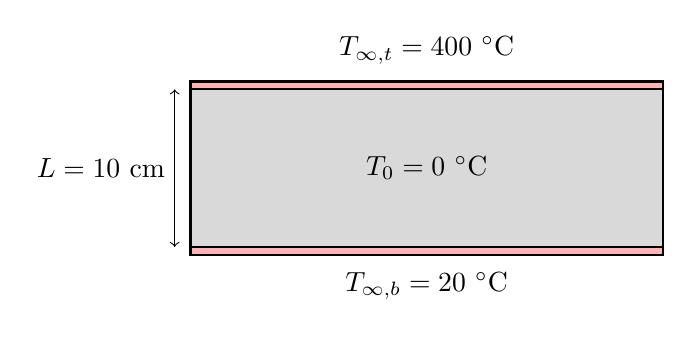
\begin{tikzpicture}[scale=1.0]
\draw[fill=gray!30,thick] (0,0) rectangle (6,2); 
\node at (3,1) {$T_0= 0~^\circ\mathrm{C}$};

\draw[fill=red!30,thick] (0,-0.1) rectangle (6,0);
\node[below] at (3,-0.2) {$T_{\infty,b} = 20~^\circ\mathrm{C}$}; 

\draw[fill=red!30,thick] (0,2) rectangle (6,2.1);
\node[above] at (3,2.2) {$T_{\infty,t} = 400~^\circ\mathrm{C}$};

\draw[<->] (-0.2,0) -- (-0.2,2);
\node[left] at (-0.2,1) {$L=10~\mathrm{cm}$};
\end{tikzpicture}
\caption{Schematic of the slab with fixed temperature boundary conditions}
\label{fig:ref_fixed_configuration}
\end{minipage}
\hfill
\begin{minipage}[t]{0.45\textwidth}
\centering
\includegraphics[width=\linewidth]{fixed_temp.png}
\caption{Comparison between numerical and analytical temperature evolution}
\label{fig:ref_fixed_temp}
\end{minipage}
\end{figure}

\ifdefined\standalone
\bibliographystyle{unsrt}
\bibliography{fixed_temp}
\end{document}
\fi






